\chapter{Обзор предметной области}
  \section{Актуальность}
    С глобальным распространением смартфонов карты стали неотъемлемой частью жизни человека, практически каждый имеет в кармане не только подробную и интерактивную карту местности, но и возможность построить маршрут до интересующей точки. Однако детализация существующих решений ограничивается автомобильными и крупными пешеходными дорогами. При этом пешеходные маршруты таких карт зачастую достаточно условны и не совпадают с реальным миром или же являются труднопроходимыми.
    Навигация внутри помещений в лучших случаях осталась в устаревшем аналоговом мире в виде указателей или же статичных бумажных карт. Современному человеку привыкшему к интерактивным картам бывает тяжело ориентироваться в незнакомом помещении.


  \section{Область применения}
    Основная область применения картографического приложения -- помощь в ориентирование на незнакомой местности, в частности на территории кампуса университета. Планировка помещений позволит легко и удобно находить не только учебный корпус, но и кабинет в нём.

    Сопутствующим продуктом разработки является высоко детализированная карта, глобальный спрос на которые растёт, например такие карты необходимы в сфере робототехники, например для автопилотируемых роботов-доставщиков Яндекс или же для точного позиционирования с использованием технологий дополненной реальности (AR).
    \begin{figure}[H]
      \centering
      \begin{subfigure}[b]{0.45\textwidth}
        \centering
        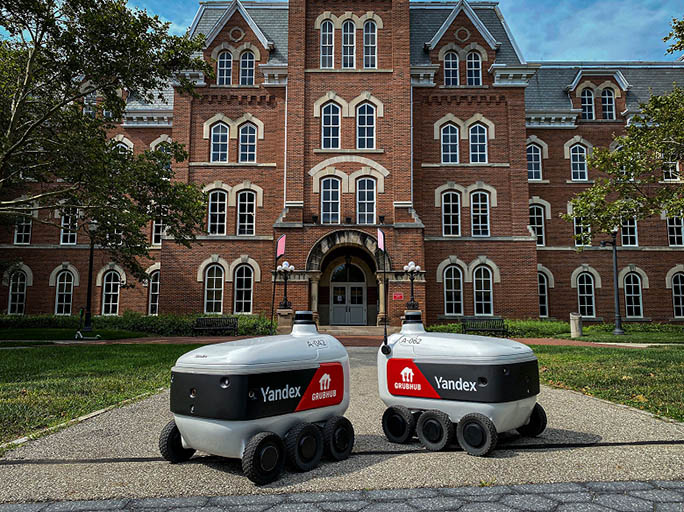
\includegraphics[width=\textwidth]{assets/img/rover.jpg}
        \caption{Ровер в университете Огайо, США}
      \end{subfigure}
      \hfill
      \begin{subfigure}[b]{.45\textwidth}
        \centering
        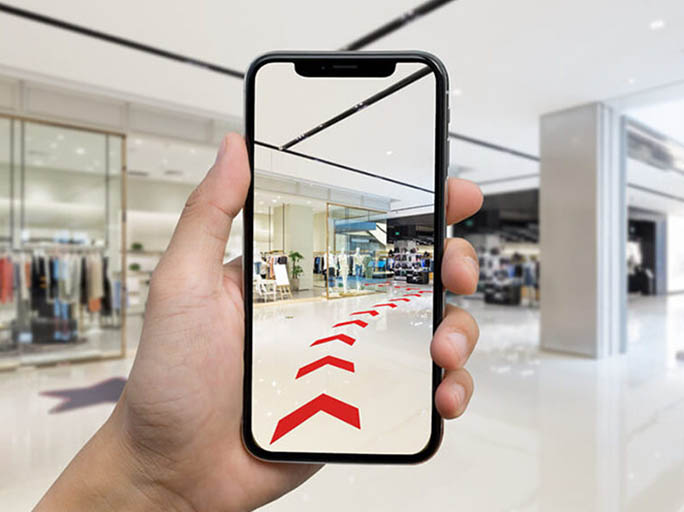
\includegraphics[width=\textwidth]{assets/img/AR.jpg}
        \caption{Навигационное приложение в AR}
      \end{subfigure}
      \caption{Примеры технологий которым необходимы высоко детализированные карты}
    \end{figure}

  \section{Обзор существующих решений}
    Проект можно разделить на 3 части:
    \begin{itemize}
      \item Детализированная карта местности
      \item Внутренняя планировка зданий
      \item Построение маршрута
    \end{itemize}


    Рассмотрим существующие решения для каждой из частей

    \subsubsection{Детализированная карта местности}
      На данный момент на рынке можно выделить два популярных приложения предоставляющих пользователям высоко детализированную карту местности: Apple Maps и 2GIS
      \paragraph{Apple Maps}
        \noindent Достоинства:
        \begin{itemize}
          \item Качественная высокая детализация автомобильных дорог и парковых зон
          \item Все примитивы карты привязаны к реальным физическим размерам. Например, дороги в классических картографических приложениях отображаются в виде линий -- ребёр графа и предоставляют пользователю информацию о том, что дорога существует, в AppleMaps дороги являются многоугольниками, демонстрируя пользователям физическую ширину дороги и пространство занимаемое ей, это позволяет легче оценивать реальную проходимость дороги
        \end{itemize}

        \noindent Недостатки:
        \begin{itemize}
          \item Высокая детализация реализована экспериментально в нескольких городах США, картография на территории России в ближайшие 5 лет не планируется
          \item Акцент сделан на автомобильные дороги, пешеходные маршруты недостаточно проработаны. Например, тротуар отображается так же, как тропинка в парке
        \end{itemize}

        \fig[Пример детализации местности Apple Maps][0.5]{assets/img/comp/apple-maps.jpg}

      \paragraph{2GIS}
        Доступна в России. Рассматривалась на примере кампуса СПбПУ
        \noindent Достоинства:
        \begin{itemize}
          \item Акцент на городах России
          \item Наивысшая достоверность среди конкурентов
        \end{itemize}

        \noindent Недостатки:
        \begin{itemize}
          \item У дорог отсутствует привязка к физической ширине, из-за чего основная аллея выглядит ровно так же, как и парковая тропинка
          \item Некоторые автомобильные дороги внутри кампуса отсутствуют
        \end{itemize}


        \fig[Пример детализации местности 2GIS][0.5]{assets/img/comp/d-gis.jpg}


    \subsubsection{Внутренняя планировка зданий}
      Многие компании владеющие популярным приложениями карт, разрабатывают свои решения для отображения на внутренней планировки зданий. Основным недостатком всех решения является отсутствие возможности строить маршрут внутри помещения.
      \paragraph{Apple Maps}
        \noindent Достоинства:
        \begin{itemize}
          \item Наиболее детализированные планы
          \item Открытый универсальный стандарт описания планов помещений. Обладает подробной документацией, стандартизирован \cite{https://www.ogc.org/standards/requests/202}
          \item Возможность добавлять свои планы в официальное приложение
        \end{itemize}

        \noindent Недостатки:
        \begin{itemize}
          \item Приоритет добавления своих планов отдан резидентам США
          \item Высокие критерии добавления своих планов (посещаемость более 1 миллиона человек в год, подходит в основном для аэропортов и вокзалов)
          \item При наличии публичного формата, отсутствует инструментарий для создания планов в этом формате. На рынке есть ряд компаний предоставляющих услуги картографии, однако эти компании не распространяют своё программное обеспечение
        \end{itemize}

        \fig[Пример планировки зданий Apple Maps][0.5]{assets/img/comp/apple-maps-indoor.jpg}

      \paragraph{Яндекс.Карты}

        \noindent Достоинства:
        \begin{itemize}
          \item Есть официальный редактор планов помещений
        \end{itemize}

        \noindent Недостатки:
        \begin{itemize}
          \item Закрытый проприетарный формат хранения планов помещений, отсутствует возможность экспорта в файл для использования в сторонних приложениях
          \item Размытая документация описывающая процесс добавления планов на карту
          \item На данным момент добавление планов на карту недоступно для произвольных зданий, новые схемы создаются по заявкам для торговых центров и вокзалов
        \end{itemize}

        \fig[Пример планировки зданий Яндекс.Карты][0.5]{assets/img/comp/yandex-indoor.jpg}

      \paragraph{2GIS Этажи}

        \noindent Достоинства:
        \begin{itemize}
          \item Яркий и контрастный дизайн
        \end{itemize}

        \noindent Недостатки:
        \begin{itemize}
          \item Карты создаются по индивидуальным заявкам
          \item Полностью отсутствует информация о процессе создания, требованиях для планов помещений, формате хранения
        \end{itemize}
        \fig[Пример планировки зданий 2GIS Этажи][0.5]{assets/img/comp/d-gis-indoor.jpg}

    \subsubsection{Построение маршрута}
      Построение маршрута по улице работает одинаково хорошо во всех популярных приложениях, однако ни одно из них не поддерживает построение маршрута внутри помещений. Существуют непубличные картографические сервисы, а так же компании разрабатывающие indoor карты под заказ с возможностью строить маршрут, однако они не вписываются в концепцию ВКР

\chapter{Требования}
  Перед началом разработки были составлены бизнес-требования в формате пользовательских историй, а так же конкретизированы общие требования разработки программного обеспечения промышленного качества

  \section{Общие требования к приложению}
    \begin{itemize}
      \item Приложение должно не противоречить принципам дизайна Apple Human Interface Guidelines для iOS \cite{HumanInterfaceGuidelines}
      \item Приложение должно поддерживать светлую и тёмную темы, переключение которых синхронизировано с системной темой операционной системы
      \item Приложение должно поддерживать все виды современных устройств на операционной системы iOS, а в частности iPhone, iPad, iPad Mini, а так же режим SplitView \cite{SplitView}.
      \item Версия приложения для планшетов должна поддерживать как портретный, так и ландшафтный режим отображения
      \item Приложение должно стабильно работать в стандартной частоте кадров устройства (120 или 60 кадров в секунду)
      \item Приложение должно поддерживать устройства с операционной системой iOS 13 и выше
    \end{itemize}

  \section{Пользовательские истории}
    \subsection{Для студентов}
      \begin{itemize}
        \item Как студент, я хочу строить маршруты до произвольного кабинета, чтобы найти деканат
        \item Как студент, я хочу видеть примерное время на маршрут, чтобы заранее оценить время пути и не опоздать на пару
        \item Как студент, я хочу искать кабинеты через поиск по ключевым словам, чтобы быстро найти местоположение кабинета на карте
        \item Как студент, я хочу видеть дополнительную информацию (адрес, телефон, почта) об объектах на карте, чтобы быстро связаться с деканатом
      \end{itemize}
    \subsection{Для гостей университета}
      \begin{itemize}
        \item Как гость отсканировавшый QR код в приглашение на мероприятие, я хочу чтобы открылась интерактивная карта с уже проложенным маршрутом, чтобы найти место проведения мероприятия
        \item Как гость пришедший на мероприятие, я хочу чтоб приложение использовало технологию AppClip, чтобы открывать его не скачивая из AppStore
      \end{itemize}
    \subsection{Для организаторов}
      \begin{itemize}
        \item Как организатор мероприятия, я хочу создавать красиво оформленные AppClip/QR коды с произвольным маршрутом без необходимости взаимодействовать с разработчиком, чтобы быстро и удобно создавать приглашения
        \item Как пользователь, я хочу быстро делиться произвольной точкой назначения с помощью ссылки, чтобы организовывать локальные встречи
      \end{itemize}

\chapter{Картография}
  При детальном рассмотрении доступных на рынке вариантов создания картографического приложения с поддержкой планов помещений, я остановился на написание своей программы, которая будет отображать карты в формате IMDF разработанным компанией Apple для Apple Maps
  \section{Формат IMDF}
    Формат Indoor Mapping Data Format (IMDF) \cite{IMDF} является обобщённой моделью описания планировок помещений, разработан компанией Apple для внутренних нужд, после чего сделан полностью свободным и бесплатным форматом при любых условиях использования. Стандартизирован Open Geospatial Consortium в 2021 году \cite{https://www.ogc.org/pressroom/pressreleases/4415}. Формат является расширением GeoJSON RFC 7946 \cite{GeoJSON RFC 7946} и полностью совместим с ним.

    \subsection{Структура IMDF}
      Согласно нотации GeoJSON, основной структурной единицей модели является Feature, модели одинакового типа складываются в массив FeatureCollection и сохраняются в формате JSON в файл с соответствующим типу модели названием.

      \subsubsection{Базовые типы}
        Нотация определяет следующие базовые типы используемые во всех моделях:
        \paragraph{LABELS}
          JSON объект используемый для обозначения одной лексической конструкции (строки) на разных языках. Пример:
          \begin{lstlisting}[language=json,caption={Пример модели LABELS}]
{
  "en": "Hello",
  "de": "Hallo"
}
          \end{lstlisting}

        \paragraph{DISPLAY-POINT}
          Используется для обозначения точечной координаты на карте в соответствие с нотацией GeoJSON
          \begin{lstlisting}[language=json,caption={Пример модели DISPLAY-POINT}]
{
  "type": "Point",
  "coordinates": [ 100.0, 0 ]
}
          \end{lstlisting}

        \paragraph{UUID}
          Уникальный внутри всего формата номер соответствующий GeoJSON FEATURE-ID, то есть являющийся строкой или числом.
          Я использую UUID v4, то есть 32х символьный номер в шестнадцатеричной системе счисления, полученный с использованием генератора случайных чисел, пример: 123e4567-e89b-12d3-a456-426614174000

        \paragraph{RESTRICTION-CATEGORY}
          Описывает возможное ограничение действующие на объект
          \begin{center}
            \begin{xltabular}{\linewidth}{|l|X|}
              \caption{Виды ограничений}\\\hline
              Категория     & Описание                                                                   \\\hline
              employeesonly & Доступ разрешен для сотрудников имеющих пропуск                            \\\hline
              restricted    & Доступ ограничен для широкой публики, однако разрешен для каких либо групп \\\hline
            \end{xltabular}
          \end{center}


      \subsubsection{Модели IMDF (Feature)}
        Вопросительный знак после типа поля означает его опциональность. Опциональные поля могут быть заполнены пустыми значениями (null) или полностью отсутствовать (undefined).

        Нотация IMDF исчерпывающи описывает следующие типы моделей (Feature), подробное описание доступно в документации\cite{IMDFFeatures}, диаграмма сущностей в приложение \ref{IMDF-ER}:
        \paragraph{Address}
          Модель используется для описывания точного почтового адреса согласно местным правовым нормам

        \paragraph{Building}
          Модель описывает структуру здания, при этом не описывая его физические границы, делегируя это модели Footprint.

          \begin{center}
            \begin{xltabular}{\linewidth}{|l|p{4cm}|X|}
              \caption{-}\\\hline
              Поле           & Тип                   & Описание                                                                                     \\ \hline
              name           & LABELS?               & Официальное название здания                                                                  \\ \hline
              alt\_name      & LABELS?               & Альтернативное название здания, которое чаще всего используется в устной речи посетителей    \\ \hline
              category       & BUILDING-CATEGORY     & Категория, которая лучше всего описывает функцию здания                                      \\ \hline
              restriction    & RESTRICTION-CATEGORY? & Категория, которая лучше всего описывает ограничение, применимое ко всему физическому зданию \\ \hline
              display\_point & DISPLAY-POINT?        & Координата используемая в качестве точечного представления здания                            \\ \hline
              address\_id    & UUID?                 & Идентификатор модели адреса (Address) этого здания                                           \\ \hline
            \end{xltabular}
          \end{center}

          Примером категории здания может служить "Учебное помещение", "Паркинг", "Магазин".

          В проекте используется для описания всех видов построек, а в частности учебных корпусов, магазинов, ресторанов, трансформаторных будок и жилых домов на территории кампуса.

    \subsection{Иерархическая структура IMDF}
      Несмотря на то, что нотация описывает модели в нормализованном формате, для лучшего понимания, следует рассматривать их как иерархическую структуру.

      \fig[Иерархическая структура представления данных][1]{assets/src/imdf-hierarchy.drawio.png}

      \begin{itemize}
        \item Самый верхний уровень представляет модель Venue это общее пространство отображаемой карты, в случае моего приложение -- весь кампус университета.
        \item Venue содержит в себе массив зданий (Building), форма которых описывается с помощью Footprint и на которые опционально ссылается модель Attraction, описывающая точки интереса.
        \item Каждое здание содержит массив этажей (Level)
        \item Каждый этаж содержит массив помещений (Unit) и детали (Detail)
        \item Каждое помещение содержит проходы (Oppening) и якоря (Anchor)
        \item На якоря ссылаются удобства (Amenity) и аннотации (Occupant)
      \end{itemize}

  \section{Расширение стандарта}
    Как видно из иерархической диаграммы, верхним уровнем формата является пространство содержащие в себе здания, структура здания исчерпывающе описана, однако нотация не предоставляет моделей для описания местности между этими зданиями внутри Venue. Тем самым стандарт захватывает часть территории, при этом позволяет описать эту территорию только зданиями, оставляя пространство между ними занятым, но пустым.
    Для решения этой проблемы, я решил расширить формат добавив в него модели описывающие местность между зданиями. Добавленные мной модели отмечены зелёным на диаграмме.

    \subsection{Описание добавленных моделей}
      \paragraph{EnvironmentUnit}
        Так как поверхность земли на улице одноэтажна, верхним уровнем можно сразу сделать модель описывающую конкретную геометрию уличных объектов.

        Модель описывает все физические пространства на улице, такие как дороги, тротуары, газон, лес, тропинки. Аналогично комнатам Unit, модель EnvironmentUnit
        \begin{center}
          \begin{xltabular}{\linewidth}{|l|p{4cm}|X|}
            \caption{Модель уличного пространства}\\\hline
            Поле           & Тип                       & Описание                                                                                 \\ \hline
            name           & LABELS?                   & Официальное название места                                                               \\ \hline
            alt\_name      & LABELS?                   & Альтернативное название места, которое чаще всего используется в устной речи посетителей \\ \hline
            category       & ENVIRONMENT-UNIT-CATEGORY & Категория, которая лучше всего описывает место                                           \\ \hline
            restriction    & RESTRICTION-CATEGORY?     & Категория, которая лучше всего описывает ограничение, применимое к месту                 \\ \hline
            display\_point & DISPLAY-POINT?            & Координата используемая в качестве точечного представления места                         \\ \hline
          \end{xltabular}
        \end{center}

        \begin{center}
          \begin{xltabular}{\linewidth}{|l|X|}
            \caption{Виды категорий EnvironmentUnit (ENVIRONMENT-UNIT-CATEGORY)}\\ \hline
            Категория              & Описание                                                                                                            \\ \hline
            road.main              & Автомобильная дорога                                                                                                \\ \hline
            road.dirt              & Неасфальтированная автомобильная дорога                                                                             \\ \hline
            road.pedestrian.main   & Основная пешеходная дорога (асфальтированный тротуар)                                                               \\ \hline
            road.pedestrian.second & Второстепенная пешеходная дорога (например асфальтированные площади, служит для контрастного отделения от основной) \\ \hline
            road.pedestrian.dirt   & Неасфальтированная  пешеходная дорога                                                                               \\ \hline
            grass                  & Область засаженная газоном                                                                                          \\ \hline
            tree                   & Область высаженных деревьев (например аллеи в парке)                                                                \\ \hline
            forest                 & Область природного леса                                                                                             \\ \hline
          \end{xltabular}
        \end{center}

      \paragraph{EnvironmentAnchor}

        Якорь представляет собой точку, используемую в качестве предпочтительного местоположения отображения определенного удобства ссылающегося на него. Связывает точку в пространстве с конкретным местом (Unit).
        \begin{center}
          \begin{xltabular}{\linewidth}{|l|p{4cm}|X|}
            \caption{Модель уличного якоря}\\\hline
            Поле     & Тип   & Описание                                     \\ \hline
            unit\_id & UUID  & Идентификатор модели места (EnvironmentUnit) \\ \hline
          \end{xltabular}
        \end{center}

      \paragraph{EnvironmentAmenity}
        Уличное удобство моделирует физическое присутствие и местоположение объекта, который служит утилитарной цели или другому удобству. Аналогичен Amenity внутри помещений.
        \begin{center}
          \begin{xltabular}{\linewidth}{|l|p{4cm}|X|}
            \caption{Модель аннотации уличного удобства}\\\hline
            Поле        & Тип                          & Описание                                                                                    \\ \hline
            name        & LABELS?                      & Официальное название удобства                                                               \\ \hline
            alt\_name   & LABELS?                      & Альтернативное название удобства, которое чаще всего используется в устной речи посетителей \\ \hline
            category    & ENVIRONMENT-AMENITY-CATEGORY & Категория удобства                                                                          \\ \hline
            detailLevel & NUMBER?                      & Уровень детализации, чем выше, тем важнее объект удобства                                   \\ \hline
            anchor\_id  & UUID                         & Идентификатор модели уличного якоря (EnvironmentAnchor)                                     \\ \hline
          \end{xltabular}
        \end{center}

        \begin{center}
          \begin{xltabular}{\linewidth}{|l|X|}
            \caption{Виды категорий EnvironmentAmenity (ENVIRONMENT-AMENITY-CATEGORY)}\\           \hline
            Категория       & Описание                                                        \\\hline
            parking.car     & Автомобильная парковка                                          \\\hline
            parking.bicycle & Велопарковка                                                    \\\hline
            banch           & Скамейка                                                        \\\hline
            entrance.public & Открытый публичный пешеходный вход (калитка)                    \\\hline
            entrance.secure & Вход по пропускам                                               \\\hline
            barrier         & Контролируемое препятствие для проезда автомобильней (шлагбаум) \\\hline
            playground      & Детская площадка                                                \\\hline
          \end{xltabular}
        \end{center}

      \paragraph{EnvironmentDetail}
        Детализация моделирует наличие, местоположение и вид физического объекта, распознавание которого в значительной степени зависит от пространственного контекста. Например дорожная разметка, перепад высот, ступеньки, заборы и т.д. Аналогичен Detail внутри помещений.
        \begin{center}
          \begin{xltabular}{\linewidth}{|l|p{4cm}|X|}
            \caption{Модель уличной детализации}\\\hline
            Поле     & Тип                         & Описание              \\ \hline
            category & ENVIRONMENT-DETAIL-CATEGORY & Категория детализации \\ \hline
          \end{xltabular}
        \end{center}

        \begin{center}
          \begin{xltabular}{\linewidth}{|l|X|}
            \caption{Виды категорий EnvironmentDetail (ENVIRONMENT-DETAIL-CATEGORY)}\\           \hline
            Категория         & Описание                                                                                             \\ \hline
            crosswalk         & Разметка пешеходного перехода                                                                        \\ \hline
            road.marking.main & Дорожная разметка (например сплошная линия между полосами )                                          \\ \hline
            parking.marking   & Разметка мест на парковке                                                                            \\ \hline
            parking.big       & Жирная разметка мест на парковке (обычно используется для запрещения парковки в определённых местах) \\ \hline
            fence.main        & Препятствие пешеходному маршруту в явно физическом виде (забор)                                      \\ \hline
            fence.heigth      & Неявное препятствие пешеходному маршруту (например резкий перепад высот)                             \\ \hline
            stpdf             & Ступеньки                                                                                            \\ \hline
          \end{xltabular}
        \end{center}

      \paragraph{Attraction}
        Точка интереса, один из видов аннотации, указывает на область сильного интереса посетителей, позволяет отображать на карте изображение, чтоб выделяться среди остальных аннотаций. Рекомендуется ассоциировать со зданиями имеющими внутреннюю планировку.
        \begin{center}
          \begin{xltabular}{\linewidth}{|l|p{4cm}|X|}
            \caption{Модель аннотации точки интересе}\\\hline
            Поле        & Тип                 & Описание                                                                                                \\ \hline
            name        & LABELS?             & Официальное название точки интереса                                                                     \\ \hline
            alt\_name   & LABELS?             & Альтернативное название точки интереса, которое чаще всего используется в устной речи посетителей       \\ \hline
            short\_name & LABELS?             & Короткое название менее чем из 2х букв для отображения внутри аннотации в случае отсутствия изображения \\ \hline
            category    & ATTRACTION-CATEGORY & Категория точки интереса                                                                                \\ \hline
            image       & URL?                & Ссылка на изображение отображаемое в аннотации                                                          \\ \hline
            building\_id& UUID?               & Идентификатор модели здания (Building) ассоциированного с этой аннотацией                               \\ \hline
          \end{xltabular}
        \end{center}
        % 
        \begin{center}
          \begin{xltabular}{\linewidth}{|l|X|}
            \caption{Виды категорий Attraction (ATTRACTION-CATEGORY)}\\           \hline
            Категория & Описание                   \\ \hline
            building  & Аннотация здания           \\ \hline
            other     & Любой другой вид аннотации \\ \hline
          \end{xltabular}
        \end{center}

    \subsection{Поиск маршрута}
      Формат IMDF не содержит в себе информации необходимой для поиска маршрута, по этому я добавил описание односвязного графа, по которому можно будет построить маршрут. Для обратной совместимости с GeoJSON, граф описывается в формате GeoJSON и состоит из двух моделей:
      \subsubsection{Модели графа маршрута}
        \paragraph{PathNode}
          Описывает вершину графа. Геометрия обязана быть Point согласно GeoJSON. Для бесшовного построения маршрута, внутри одного графа, вершины могут находиться как на улице, так и в помещение, для верного отображения маршрута, каждая вершина обладает информацией о своём нахождение. Для вершин внутри зданий, указывается идентификатор модели здания (Building) и этажа (Level) на котором находится вершина.
          \begin{center}
            \begin{xltabular}{\linewidth}{|l|p{4cm}|X|}
              \caption{Модель вершины графа маршрутов}\\\hline
              Поле        & Тип                   & Описание                                                                                                                                                                    \\ \hline
              builing\_id & UUID?                 & Идентификатор модели здания (Building) в котором находится вершина                                                                                                          \\ \hline
              level\_id   & UUID?                 & Идентификатор модели этажа (Level) в котором находится вершина                                                                                                              \\ \hline
              neighbours  & UUID[]                & Массив идентификатор соседних вершин в которые можно перейти                                                                                                                \\ \hline
              weights     & NUMBER[]?             & Массив коэффициентов весов для перехода к соседним вершинам, длинна массива обязана совпадать с длинной массива neighbours. Если массив не указан, используется массив из 1 \\ \hline
              category    & PATH-NODE-CATEGORY    & Категория вершины (используется для поиска маршрута с учётом параметров)                                                                                                    \\ \hline
              restriction & RESTRICTION-CATEGORY? & Категория описывающая применимое к вершине ограничение (используется для поиска маршрута с учётом параметров)                                                               \\ \hline
            \end{xltabular}
          \end{center}

          \begin{center}
            \begin{xltabular}{\linewidth}{|l|X|}
              \caption{Виды категорий PathNode (PATH-NODE-CATEGORY)}\\             \hline
              Категория   & Описание                      \\ \hline
              crosswalk   & Разметка пешеходного перехода \\ \hline
              stairs      & Ступеньки                     \\ \hline
              dirt        & Неасфальтированная дорога     \\ \hline
              indoor.main & Маршрут внутри помещения      \\ \hline
            \end{xltabular}
          \end{center}


        \paragraph{PathNodeAssociated}
          Перед поиском маршрута необходимо определить начальную и конечную вершину графа, для этого необходимо связать вершины графа с отображаемыми пользователю аннотациями, для этой задачи служит модель PathNodeAssociated.
          \begin{center}
            \begin{xltabular}{\linewidth}{|l|p{4cm}|X|}
              \caption{Модель ассоциации вершин графа маршрутов с аннотациями}\\\hline
              Поле            & Тип  & Описание                                                                                                             \\ \hline
              path\_node\_id  & UUID & Идентификатор модели вершины маршрута (PathNode)                                                                     \\ \hline
              associeted\_id  & UUID & Идентификатор модели аннотации (Occupant/Amenity/Attraction/EnvironmentAmenity) ассоциированной с указанной вершиной \\ \hline
            \end{xltabular}
          \end{center}


          Если аннотация ассоциирована более чем с одной точкой маршрута (это может случиться с кабинетом у которого несколько входов), тогда система поиска маршрута рассмотрит все варианты и выберет кратчайший путь.

  \section{Конструктор расширенного стандарта}
    Несмотря на открытость формата и его мировую стандартизацию, открытого программного обеспечения для создания карт в этом формате нет, тем более нет программного обеспечения для моей расширенной версии формата, по этому я разработал свой собственный конструктор карт. Конструктор, на данный момент, не является конечным программным продуктом, и создан исключительно для решения утилитарной задачи -- быстро и легко нарисовать карту. Конструктор написан на языке C\# и использует возможности редактора Unity3D \cite{Unity3D}, а в частности редактор полигонов, иерархическую систему хранения объектов, компонентный подход к разработке, инспектор для редактирования параметров компонентов.

    Было разработано дополнительное окно редактора для быстрого создания IMDF объектов, разработаны компоненты представляющие все основные модели формата, написана система сериализации в IMDF. В конструкторе планировка представляется в виде иерархической структуры, что сильно ускоряет её создание. Например, комнаты Unit являются дочерними к этажу Level, которые дочерние к зданию Building. При сериализации, иерархическая структура нормализуется и все необходимые ссылки устанавливаются автоматически, кроме того по умолчанию комнаты Unit "наследуют" адрес здания дописывая к нему своё название, что позволяет явно не указывать большую часть параметров формата. Для аннотаций создан отдельный компонент, которые объединяет в себе логику аннотации (Occupant) и якоря (Anchor), что значительно ускоряет процесс их размещения на карте.

    Отдельно реализован инструмент для прокладывания графа маршрута с возможностью связать новую вершину с ближайшей или прошлой вершиной, кроме того, при добавлении ребра, по умолчанию инструмент делает его двунаправленным, то есть переход возможен в обе стороны.

    [Скриншот конструктора IMDF формата](Картинка)

    После сериализации получается полностью корректный формат IMDF расширенный моделями окружения. Обратная совместимость с форматом IMDF и базовым GeoJSON соблюдена.

  \section{Оцифровка карты}
    Процесс создания карты заключается в представление физических особенностей местности в форме многоугольников. Для увеличения продуктивности, конструктор позволяет привязать картинку к географическим координатам и отобразить на фоне редактора. В качестве первого приближения можно использовать снимки из космоса, однако они обладают рядом недостатков:
    \begin{itemize}
      \item низкое разрешение
      \item перспективные искажения, из-за которых высокие здания получаются сдвинутыми относительно фундамента
      \item кроны деревьев, которые полностью перекрывают пешеходные дорожки
    \end{itemize}

    \subsection{Ортофотоплан}
      Для нивелирования недостатков снимков из космоса, я решил составить ортофотоплан кампуса университета. Это цифровое трансформированное изображение местности, созданное по перекрывающимся исходным фотоснимкам. Для фотоснимков использовался квадрокоптер DJI Mavic 2 Zoom.
      С помощью программы Copterus \cite{Copterus} был составлен полётный план со следующими параметрами:

      \begin{itemize}
        \item высота полёта: 120м
        \item горизонтальное перекрытие: 85\%
        \item вертикальное перекрытие: 70\%
      \end{itemize}

      Было получено 1100 фотографий, которые впоследствии были обработаны программой WebODM \cite{WebODM}. В результате получен ортофотоплан кампуса с разрешением 5см в каждом пикселе ()\ref{appendix:graph}.

      [Картинка в приложение](Приложение)

\chapter{Разработка приложения}
  Разработка приложение велась в среде Xcode. Был использован язык программирования Swift. В качестве архитектурного паттерна для разработки приложения был выбран Cacao MVC, это классический подход к разработке приложений для iOS, наиболее простой способ написания кода, который поддерживается абсолютным большинство библиотек, также приложения с таким паттерном проще и дешевле поддерживать, потому что есть много специалистов умеющих им пользоваться.

  \section{Пользовательский интерфейс}
    В разработке под iOS есть несколько вариантов верстки пользовательского интерфейса, важно перед началом разработки выбрать один из них и вести разработку в нём, так как переключиться по ходу разработки будет проблематично. Рассмотрим преимущества и недостатки каждого подхода

    \paragraph{Storyboard}
      Базовый подход к созданию интерфейса, заключается в создание интерфейса с помощью специального конструктора в Xcode путём перетаскивания блоков на экран устройства. После запуска интерфейс конвертируется в UIKit объекты, к которым можно получить доступ с помощью специальных связок @IBOutlet

      \noindent Достоинства:
      \begin{itemize}
        \item наглядность
      \end{itemize}

      \noindent Недостатки:
      \begin{itemize}
        \item сложность отслеживания изменений (файл интерфейса автосгенерированный xml код)
        \item сложность контроля через код
        \item сложно переиспользовать компоненты
      \end{itemize}



    \paragraph{Написание интерфейса кодом}
      Подход похожий на Storyboard, однако подразумевает "ручное" создание UIKit объектов и размещение их друг относительно друга

      \noindent Достоинства:
      \begin{enumerate}
        \item каждый элемент интерфейса является обычным объектом языка, что позволяет в любой момент получить к нему доступ
        \item легко отслеживать изменения
        \item полный контроль над интерфейсом
        \item простота переиспользования компонентов
      \end{enumerate}

      \noindent Недостатки:
      \begin{itemize}
        \item описание интерфейса занимает очень много кода
        \item отсутствует предпросмотр интерфейса, визуально можно оценить результат только после компиляции и запуска на устройстве
      \end{itemize}


    \paragraph{SwiftUI}
      Библиотека для написания интерфейса с помощью декларативного кода

      \noindent Достоинства:
      \begin{itemize}
        \item малое количество кода даёт большой результат
        \item простота переиспользования компонентов
        \item предпросмотр интерфейса
      \end{itemize}
      \noindent Недостатки:
      \begin{itemize}
        \item на данный момент не полностью покрывает UIKit, и на решение многих примитивных задач потребуются много времени
        \item недостаточный контроль над интерфейсом
      \end{itemize}


  \section{Структурные части пользовательского интерфейса}
    Пользовательский интерфейс моего приложения можно разделить на следующие части
    \begin{itemize}
      \item отображение карты
      \item отображение информации о выбранном объекте на карте
      \item вспомогательные всплывающие окна несвязанные с картой (например окно поделиться маршрутом)
    \end{itemize}

    В результате анализа, для разработки основной части интерфейса приложения был выбран способ написания его с помощью кода, однако для вспомогательных всплывающих окон, которые не имеют зависимостей в основной части интерфейса, используется SwiftUI. Такой подход позволил иметь полный контроль над картой и основной логикой приложения, однако оставил простоту написания для "одностраничных" независимых вспомогательных окон


  \section{Чтение формата IMDF}
    Формат GeoJSON, который является базой IMDF, не подразумевает строгой типизации моделей, это делает десереализацию такого формата в строго типизированном языке нетривиальной задачей. Стандартный фреймворк для работы с картами MapKit поддерживает десереализацию идентификаторов (identifier) и геометрии (geometry) объектов GeoJSON в класс MKGeoJSONFeature, однако полезную нагрузку (properties) необходимо получать самостоятельно.

    \begin{lstlisting}[language=swift,caption={Интерфейс объекта MKGeoJSONFeature}]
open class MKGeoJSONFeature : NSObject, MKGeoJSONObject {
  open var identifier: String? { get }
  open var properties: Data? { get }
  open var geometry: [MKShape & MKGeoJSONObject] { get }
}
  \end{lstlisting}

    Для универсальной десереализации всех моделей был создан класс Feature шаблонизируемый классом Properties, конструктор класса сохраняет идентификатор и геометрию из MKGeoJSONFeature и декодирует Data в Properties

    \begin{lstlisting}[language=swift,caption={Реализация класса Feature}]
class Feature<Properties: Decodable>: NSObject, IMDFDecodableFeature {
let identifier: UUID
let properties: Properties
let geometry: [MKShape & MKGeoJSONObject]

required init(feature: MKGeoJSONFeature) throws {
    identifier = UUID(uuidString: feature.identifier!)!
    geometry = feature.geometry

    if let propertiesData = feature.properties {
        properties = try JSONDecoder().decode(Properties.self, from: propertiesData)
      } else {
        throw IMDFError.invalidData
      }

    super.init()
  }
}
  \end{lstlisting}

    Модели IMDF необходимо наследовать от Feature передавая в качестве шаблона десереализуемую структуру Properties

    \begin{lstlisting}[language=swift,caption={Пример объявления модели Unit}]
class Unit: Feature<Unit.Properties> {
    enum Category: String, Codable { ... }

    struct Properties: Codable {
        let name: LocalizedName?
        let alt\_name: LocalizedName?

        let level\_id: UUID
        let category: Category
        let restriction: Restriction?
        let display\_point: PointGeometry?
    }
}
    \end{lstlisting}

    Для десереализации FeaturesCollection была написана функция decodeFeatures, с её помощью можно получить типизированный массив моделей

    \begin{lstlisting}[language=swift,caption={Пример десереализации массива комнат Units}]
let imdfUnits = try decodeFeatures(Unit.self, path: unitPath)
static func decodeFeatures<T: IMDFDecodableFeature>(type: T.Type, path: URL) throws -> [T] {
let data = try Data(contentsOf: path)
let geoJSONFeatures = try MKGeoJSONDecoder().decode(data)

guard let features = geoJSONFeatures as? [MKGeoJSONFeature] else {
   throw IMDFError.invalidType 
}
let imdfFeatures = try features.map { try type.init(feature: $0) }
  \end{lstlisting}

  \section{Отображение карты}
    Есть два способа отображения карты:
    \begin{itemize}
      \item использовать картографический фреймворк с возможностью добавления своих элементов наложения (оверлея). Есть несколько таких фреймворков:
      \item MapKit официальный фреймворк Apple, позволяет отображать векторную геометрию наложения, а так же аннотации. Поддерживает многопоточную отрисовку, а так же кеширования аннотаций для последующего переиспользования
      \item YandexMapKit фреймворк компании Яндекс позволяющий отображать Яндекс карты, добавлять на них аннотации. Сильно ограничен лицензионным соглашением и обладает плохой документацией
      \item MapBox iOS SDK предоставляет доступ к картам OpenStreetMap, добавление наложения сильно ограничено. Для полноценного отображения карты необходимо загружать её на сервера MapBox
      \item отображать карту с помощью фрейморка низкоуровневой отрисовки графики Core Graphics. Данный способ наиболее универсален, но при таком подходе придётся полностью писать код для взаимодействия с вводом пользователя, придётся реализовывать жесты приближения и вращения карты, а так же оптимизировать производительность отображения наложений и аннотаций.
    \end{itemize}


    Был выбран оптимальный с точки зрения сложности реализации и качества результата фреймворк MapKit от компании Apple, несмотря на некоторые сложности в отображение наложений, он уже предоставляет готовые механизмы взаимодействия с картой. Кроме того, готовый фрейморк позволяет отображать наложения поверх обычной карты города благодаря чему, высоко детализированный кампус органично впишется в общую карту.

    \subsection{Отображение наложений на карту}
      После десереализации с помощью MKGeoJSONDecoder, геометрия представляется в виде массива композиции [MKShape \& MKGeoJSONObject]

      \fig[Диаграмма классов GeoJSON.geometry][1]{assets/src/imdf-shape.drawio.png}

      Объекты геометрии полученные после декодирования удовлетворяют интерфейсу MKOverlay. После добавление на экран MKMapView, с помощью функции \textit{addOverlay(\_ overlay: MKOverlay)} можно добавить геометрию для отображения на карте. После чего в делегате MKMapViewDelegate необходимо переопределить функцию \textit{mapView(\_ mapView: MKMapView, rendererFor overlay: MKOverlay) -> MKOverlayRenderer}, которая для каждого объекта геометрии должна вернуть потокобезопасный экземпляр MKOverlayRenderer. Фреймворк предоставляет готовые реализации MKOverlayRenderer для всех видов геометрии. Во время разработки я столкнулся с проблемой, что векторное отображение возможно только при использовании готовых реализаций, из-за этого возникают серьёзные проблемы с кастомизанией, например для MKLineRenderer невозможно указать цвет обводки.
      Для базовой кастомизации я сделал интерфейс Styleble, который реализуют все виды наложения. Функция \textit{configurate(\_ renderer: MKOverlayRenderer)} позволяет делегировать объектам карты конфигурацию компонента отрисовки.

      \fig[Диаграмма классов объектов наложение][1]{assets/src/imdf-objects-configurate.drawio.png}

      После чего, в функции делегата можно создать новый экземпляр MKOverlayRenderer, и сконфигурировать его приведя MKOverlay к интерфейсу Styleble

      \begin{lstlisting}[language=swift,caption={Реализация функции создания и конфигурации компонентов MKOverlayRenderer}]
func renderer(for overlay: MKOverlay) -> MKOverlayRenderer {
  switch overlay {
      case is MKMultiPolygon: return MKMultiPolygonRenderer(overlay: overlay)
      case is MKPolygon: return MKPolygonRenderer(overlay: overlay)
      case is MKMultiPolyline: return MKMultiPolylineRenderer(overlay: overlay)
      case is MKPolyline: return MKPolylineRenderer(overlay: overlay)
      default: return MKOverlayRenderer(overlay: overlay)
    }
}

func mapView(_ mapView: MKMapView, rendererFor overlay: MKOverlay) -> MKOverlayRenderer {
    let renderer = renderer(for: overlay)
    (overlay as? Styleble)?.configurate(renderer: renderer)

    return renderer
}
      \end{lstlisting}

    \subsection{Отображение аннотаций на карте}
      Аннотации это текстовые сообщения, привязанные географическим координатам на карте. Добавляются на карту аналогично оверлею, фреймворк автоматически кеширует и переиспользует аннотации одного типа. Аннотации представляют собой UIView аналогичные тем, что используются для отображения всего остального интерфейса в UIKit.
      В моём приложении реализовано три типа аннотаций:
      \begin{itemize}
        \item OccupantAnnotation -- используется для отображения аннотаций занимающих кабинеты, при выборе увеличивается и показывает пиктограмму категории аннотации. Например: учебный кабинет, лекторий, туалет
        \item AmenityAnnotation -- используется для отображения удобств. Например: лестница, вендинговый аппарат, парковка
        \item AttractionAnnotation -- используется для отображения точек интереса. Например: Главное здание
      \end{itemize}

      % \fig[Реализованные типы аннотаций][1]{assets/src/app-links.drawio.png}
      % TODO: 

      Все аннотации поддерживают четыре вида размеров: скрыт, маленький, нормальный, большой. Определение размера относительно приближения карты делегируются экземпляру объекта DetailLevelProcessor, благодаря этому один тип аннотации может обладать разным уровнем детализации в зависимости от представляемого вида объекта. Кроме того каждая аннотация может находиться в состояние "выбрана" и в состояние "закреплена". Для переходов между всеми комбинациями состояний предусмотрены анимации.

      % \fig[Пример отображения разных состояний OccupantAnnotation][1]{assets/src/app-links.drawio.png}
      % TODO: 

  \section{Интернационализация}
    Так как после смены языка операционная система принудительно перезапускает приложение, механизма для смены языка во время работы приложения делать не нужно.

    \subsubsection{Локализация текстов}
      В XCode встроен готовый механизм локализации с помощью создания файлов Localizable.strings, который представляет собой структуру "ключ = значение;", чтобы получить локализованную строку, необходимо использовать let value = NSLocalizedString(key: "key") \cite{NSLocalizedString}. Такой подход плох тем, что ключи передаются в строковом виде, и в случае отсутствия ключа в файле локализации случится ошибка времени выполнения. Для переноса обнаружения ошибки на время компиляции я использую библиотеку SwiftGen \cite{SwiftGen} распространяемую по лицензии MIT \cite{MIT}, которая по файлу локализации генерирует статический класс, через который можно получить доступ только к тем значениям, которые точно есть в файле локализации. Пример использования: let value = L10n.key.

    \subsubsection{Локализация карты}
      Формат IMDF подразумевает хранение всех строковых представлений с помощью LABELS, которое представляет собой словарь [язык:строка]. Это значит что файл карты уже содержит все нужные локализации, и остаётся в момент десереализации выбрать нужную в зависимости от текущей локали приложения.

    \subsubsection{Локализация значений}
      В подробной информации о маршруте отображаются его расстояние и время на прохождение, в зависимости от локали пользователя должны отличаться единицы измерения расстояния, десятичный разделитель, локализация единиц измерения. Для решения этой задачи я использую встроенные в язык программирования MKDistanceFormatter \cite{MKDistanceFormatter} и DateComponentsFormatter \cite{DateComponentsFormatter} для форматирования дистанции и времени в строки с учётом текущей локали.

  \section{Адаптивные цвета}
    Для удовлетворения поставленным требованиям, в приложение было необходимо сделать поддержку переключения между тёмной и светлой темами. Это означает, что для каждого элемента интерфейса необходимо определить два варианта цвета, и переключаться между ними во время изменения системой темы оформления. В большинстве случаев для этого достаточно использовать стандартный компонент UIColor, а цвета создавать в формате ассетов XCode, это позволяет присвоить цветам названия, и для каждого цвета указать его варианты для светлой и тёмной темы, при изменении систменой темы, варианты цвета будут изменяться автоматически. Кроме того, для многих задач следует использовать стандартные системные цвета, доступные как статические поля класса UIColor. Например, для текста следует использовать UIColor.label [Полный список системных цветов](https://sarunw.com/posts/dark-color-cheat-sheet/)
    Используемая для локализации библиотеки SwiftGen, также генерирует класс с типизированным списком всех ассетов цветов, что позволяет решить проблему с получением ассета цвета по строковому ключу.

  \section{Оптимизация процесса разработки}
    В качестве системы контроля версий использовался GitHub, разработка велась согласно GitFlow. Для упрощения процесса тестирования и распространения тестовых версий использовался TestFlight. Был написан CI/CD использующий GitHub Actions, который на каждое изменение ветки dev, производил компиляцию проекта, подписывал её сертификатами и отправлял на сервера в TestFlight, после чего тестовая сборка "по воздуху" устанавливалась на все устройства тестировщиков. Для упрощения процесса компиляции и отправки была использована платформа Fastlane \cite{Fastlane}.

    Стоит отметить, что репозиторий с приложением публичен, а для подписывания сборки необходимо использовать приватные сертификаты разработчика, которые в публичном репозитории не хранятся. Для решения этой проблемы был создан приватный репозиторий с сертификатами, которые скачиваются на CI сервер во время выполнения сборки, пароль для доступа к этому репозиторию хранится в специальном хранилище Github Secrets, значения из которого можно безопасно использовать в Action публичных репозиториев.

\chapter{Функция поделиться}
  Одна из важных особенностей любого картографического приложения это возможность поделиться маршрутом. В моём приложении для этого предусмотрена возможность поделиться URL ссылкой на маршрут. После прокладывания маршрута, можно через меню "поделиться" получить ссылку на маршрут. Кроме того к маршруту можно добавить приветственное сообщение, которое отобразится при открытии ссылки. Через это же меню можно создать красивый QR или AppClip коды.

  \section{Universal Links}
    Для того чтобы на устройствах iOS ссылка открывалась не в браузере, а в приложение, была интегрирована технологии Universal Links \cite{UniversalLinks}. Для этого была включена поддержка ассоциации с доменами (Associated Domains) на портале разработчика, а так же в проекте Xcode в соответствующем разделе указан ассоциированный домен. После чего, при открытии ссылки, операционная система перенаправит пользователя на приложение, при этом передав ссылку в параметр userActivity у AppDelegate

    \begin{lstlisting}[language=swift,caption={Получение ссылки из Universal Links}]
func application(\_ application: UIApplication, continue userActivity: NSUserActivity, restorationHandler: [Any?] -> Void) -> Bool {
  guard userActivity.activityType == NSUserActivityTypeBrowsingWeb, let url = userActivity.webpageURL else { return false }

  print(url)
  return true
}
    \end{lstlisting}

  \section{AppClip}
    Наиболее распространённый случай использования ссылок на маршрут это размещение их в приглашениях на мероприятия, целевая аудитория таких приглашения -- гости университета, у которых, вероятнее всего, приложение не будет установленно на устройтсво и Universal Links не сработает. Для таких случаев в моём приложении предусмотрена технология блиц-приложений AppClip \cite{AppClip}.
    Блиц-приложение это отдельная версия программы, с помощью которой пользователь может получить быстрый доступ к определённым функциям приложения, при этом загрузка и установка полной версии из магазина приложений не требуется.
    Для блиц-приложение есть несколько вариантов запуска
    \begin{itemize}
      \item поднести устройство к NFC-метке
      \item отсканировать фирменную метку App Clip или стандартный QR-код
      \item перейти по URL ссылке в Safari, «Сообщениях» и других сервисах Apple
      \item запустить из баннера на сайте
      \item открыть предложенный App Clip в Apple Maps
      \item воспользоваться банером "предложения Siri" на основе местоположения пользователя
    \end{itemize}


    После наступления одного из событий, операционная система отображает банер с предложением перейти в приложение, поле того как пользователь соглашается, мгновенно открывается упрощённая версия программы, в которую при наличии передаётся ссылка методом Universal Links.

      [Картинка работы AppClip](Картинка)

    В случае если пользователь выйдет из приложения, повторно открыть его можно будет через специальный ярлык, который будет существовать ещё несколько недель, после чего автоматически удалится.

  \section{Описание использования}
    Любой пользователь через установленное приложение может создать URL ссылку на маршрут и поместить её в QR или AppClip код, после чего, например, поместить в приглашение на мероприятие. Любой пользователь отсканировавший код, или перешедший по ссылке увидит этот маршрут на интерактивной карте.
    Если ссылка была открыта не на устройстве iOS, то откроется сайт с информацией о маршруте, иначе с использованием Universal Links будет открыта основная версия приложения, если она есть на устройстве или будет установлена и открыта блиц версия. После открытия будет проложен маршрут и отобразиться окно с информацией о нём.

    \fig[Алгоритм открытия ссылки][1]{assets/src/app-links.drawio.png}

\chapter{Серверная часть}
  Для поддержки системы "поделиться маршрутом"\ и ещё некоторых незначительных функций приложения необходим веб сервер. Для приложения был зарегистрирован домен polymap.ru и разработан веб сервер с использованием языка NodeJS \cite{NodeJS} и фреймворка Express \cite{Express}. Через Let’s Encrypt \cite{Let’s Encrypt} были получены SSL сертификаты для поддержки протокола HTTPS.

  \subsubsection{Ассоциация домена с приложением}
    Для корректной работы Universal Links и AppClip необходимо ассоциировать приложение с доменом. Это означает, что на GET запрос по пути https://polymap.ru/.well-known/apple-app-site-association, должен вернуться текстовый файл, в котором должны быть записаны данные об ассоциации приложения в формате JSON. При этом сервер должен поддерживать протокол https. Пример файла:

    \begin{lstlisting}[language=json,caption={Файл ассоциации домена с приложением}]
{
  "applinks": {
    "details": [
      {
        "appIDs": [ "ABCDE12345.com.example.app" ],
        "paths": ["/"]
      }
    ]
  }
}
  \end{lstlisting}

    Для поддержки AppClip в вышеуказанный файл необходимо добавить соответствующий раздел:

    \begin{lstlisting}[language=json,caption={Ассоциация домена с AppClip}]
{
  ...
  "appclips": {
    "apps": ["ABCED12345.com.example.MyApp.Clip"]
  }
}
  \end{lstlisting}

    В момент открытия ссылки пользователем и наличие приложения ассоциированного с этой ссылкой, операционная система обращается к серверам Apple, которые обращаются к корневому домену ссылки и проверяют наличие ассоциации с приложением. Эта проверка кешируется на серверах Apple на 24 часа, что полностью снимает нагрузку с пользовательских серверов.

    \fig[Диаграмма взаимодействия при открытии ссылки][1]{assets/src/open-url.drawio.png}

  \subsubsection{Поддержка функции поделиться}
    Для того чтоб поделиться маршрутом необходимо передать следующие параметры:
    \begin{itemize}
      \item UUID начала маршруту
      \item UUID завершения маршрута
      \item Параметры построения маршрута
      \item Разрешение менять параметры
      \item Приоритет асфальтированным маршрутам
      \item Разрешение служебных проходов
      \item Приветственное сообщение
    \end{itemize}

    Технически все эти параметры можно поместить в часть qurey параметров URL, однако тогда ссылка получится длинной и отпугивающей пользователя, кроме того, QR код для длинной ссылки потребует высокой детализации, что означает более долгое сканирование и менее привлекательный вид. AppClip код и вовсе позволяет закодировать около 50 символов, некоторые сочетания которых кодируются оптимальнее, однако длинную ссылку с несколькими UUID закодировать точно не получится.
    ![Пример QR кода для ссылок разной длины]()
    ![20 символов]()
    ![80 символов]()

    Для сокращения ссылки была разработана следующая система: пользователь POST запросом отправляет на сервер все параметры связанные с маршрутом, они сохраняются в базу данных, а пользователю отдаётся ID этой записи. После чего пользователь может сделать запрос на сервер с указанным ID и получить сохранённые параметры маршрута.

    \paragraph{Генерация AppClip кодов}
      Сложность генерации AppClip кодов состоит в том, что это закрытый формат представления данных и получить этот код можно только с помощью специальной CLI программы \cite{AppClipGenerator}, существующей только для системы MacOS. Из-за этого сгенерировать AppClip код прямо на устройстве не возможно, по этому генерация кода была вынесена на сервер. GET запрос на адрес polymap.ru/api/appclip-code генерирует и возвращает AppClip код, принимая следуюшие query параметры:
      \begin{center}
        \begin{xltabular}{\linewidth}{|l|p{3cm}|X|}
          \caption{Поддерживаемые query параметры генератора AppClip кодов}\\\hline
          Параметр       & Пример & Описание                                                     \\ \hline
          id             & 5      & ID кода                                                      \\ \hline
          background     & fff    & Цвет фона в формате HEX                                      \\ \hline
          primary        & 000    & Основной цвет в формате HEX                                  \\ \hline
          secondary      & 888    & Второстепенный цвет в формате HEX                            \\ \hline
          badgeTextColor & 888    & Цвет текста в формате HEX                                    \\ \hline
          logo           & camera & Ваиант логотипа в центре кода. [camera, nfc]                 \\ \hline
          useBadge       & true   & Разрешить использовать рамку вокург кода                     \\ \hline
          type           & 888    & Тип файла [svg, png]                                         \\ \hline
          width          & 512    & В случе png изображения его ширина в пиксилях. Максимум 2048 \\ \hline
        \end{xltabular}
      \end{center}


      С помощью этих параметров можно полностью кастомизировать код и получить любой из возможных его вариантов.

      Так как сервер запускается на операционной системе Linux, а программа для генерации существует только для MacOS, смысловая нагрузка когда, прерывистые окружности, в формате SVG предгенерирована на MacOS для каждого варианта ID, сервер берёт нужный файл и оформляет код согласно пришедшем параметрам. Данное решение уникально и не встречается ни в одном другом приложении.

      \fig[Схема работы диалога поделиться][1]{assets/src/share.drawio.png}

